
\documentclass[tikz, border=10mm]{standalone}
\usepackage{xcolor}
\usepackage{tikz}
\usetikzlibrary{positioning, calc, backgrounds, quotes, arrows.meta}

% Color Definitions (Matching nn_blocks.tex)
\definecolor{ConvColor}{rgb}{0.98,0.81,0.69}
\definecolor{PoolColor}{rgb}{0.8,0.33,0.33}
\definecolor{UnpoolColor}{rgb}{0.6,0.7,0.9}
\definecolor{ResBlockColor}{rgb}{0.85,0.92,1.0}
\definecolor{OpColor}{rgb}{0.5,1.0,0.5}
\definecolor{FcColor}{rgb}{0.6,0.2,0.8}
\definecolor{SoftmaxColor}{rgb}{0.9,0.9,0.6}
\definecolor{EmbedColor}{rgb}{0.95,0.95,0.8}
\definecolor{TransColor}{rgb}{0.8,0.9,0.8}

% 2D Style (Flowchart)
\tikzset{
    layer/.style={
        rectangle,
        rounded corners=1mm,
        minimum height=2.0em,
        minimum width=3.0em,
        align=center,
        draw=black!80,
        thick
    },
    conv/.style={layer, fill=ConvColor},
    pool/.style={layer, fill=PoolColor},
    up/.style={layer, fill=UnpoolColor},
    res/.style={layer, fill=ResBlockColor},
    op/.style={layer, fill=OpColor},
    fc/.style={layer, fill=FcColor},
    softmax/.style={layer, fill=SoftmaxColor},
    embed/.style={layer, fill=EmbedColor},
    trans/.style={layer, fill=TransColor},
    relu/.style={layer, fill=yellow!10, draw=yellow!80!black},
    io/.style={circle, minimum width=3.0em, draw=black!80, fill=gray!20, thick, align=center},
    skip/.style={->, dashed, draw=blue!60, thick},
    arrow/.style={->, very thick, draw=black!80, rounded corners=0.2cm}
}

\begin{document}
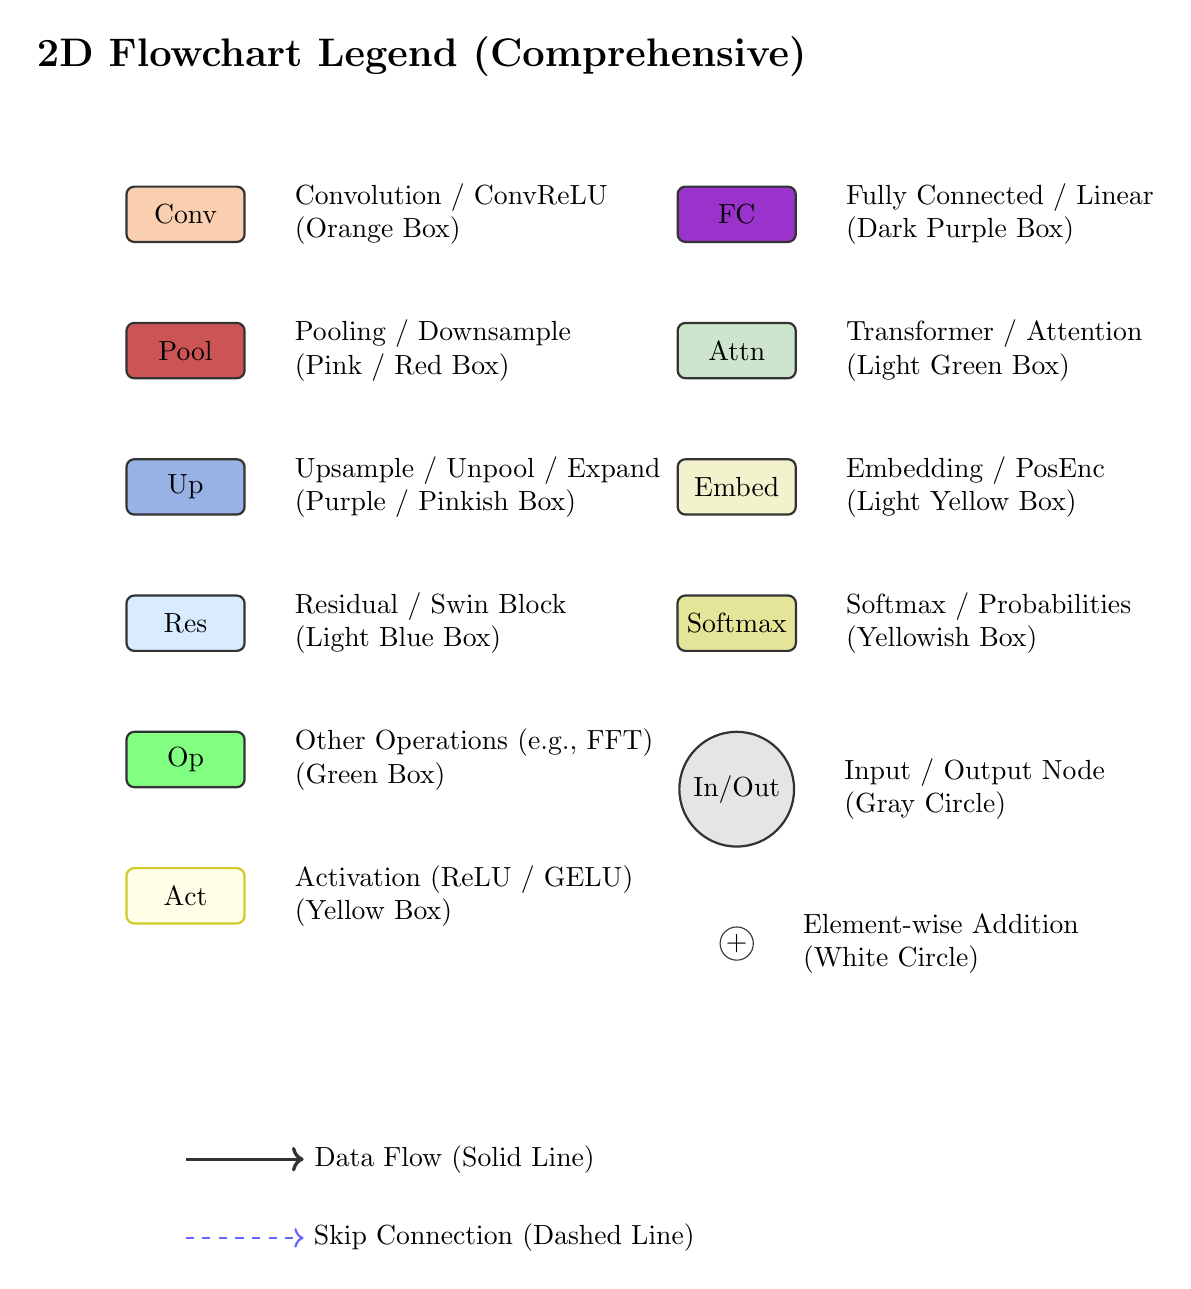
\begin{tikzpicture}[node distance=0.8cm, every node/.style={transform shape}]

% Title
\node[font=\Large\bfseries] at (3, 9.5) {2D Flowchart Legend (Comprehensive)};

% Column 1
\coordinate (col1) at (0, 7.5);

\node[conv, minimum width=1.5cm] (n_conv) at (col1) {Conv};
\node[right=0.5cm of n_conv, align=left] {Convolution / ConvReLU\\(Orange Box)};

\node[pool, minimum width=1.5cm, below=1.0cm of n_conv] (n_pool) {Pool};
\node[right=0.5cm of n_pool, align=left] {Pooling / Downsample\\(Pink / Red Box)};

\node[up, minimum width=1.5cm, below=1.0cm of n_pool] (n_up) {Up};
\node[right=0.5cm of n_up, align=left] {Upsample / Unpool / Expand\\(Purple / Pinkish Box)};

\node[res, minimum width=1.5cm, below=1.0cm of n_up] (n_res) {Res};
\node[right=0.5cm of n_res, align=left] {Residual / Swin Block\\(Light Blue Box)};

\node[op, minimum width=1.5cm, below=1.0cm of n_res] (n_op) {Op};
\node[right=0.5cm of n_op, align=left] {Other Operations (e.g., FFT)\\ (Green Box)};

\node[relu, minimum width=1.5cm, below=1.0cm of n_op] (n_act) {Act};
\node[right=0.5cm of n_act, align=left] {Activation (ReLU / GELU)\\(Yellow Box)};

% Column 2
\coordinate (col2) at (7, 7.5);

\node[fc, minimum width=1.5cm] (n_fc) at (col2) {FC};
\node[right=0.5cm of n_fc, align=left] {Fully Connected / Linear\\(Dark Purple Box)};

\node[trans, minimum width=1.5cm, below=1.0cm of n_fc] (n_trans) {Attn};
\node[right=0.5cm of n_trans, align=left] {Transformer / Attention\\(Light Green Box)};

\node[embed, minimum width=1.5cm, below=1.0cm of n_trans] (n_embed) {Embed};
\node[right=0.5cm of n_embed, align=left] {Embedding / PosEnc\\(Light Yellow Box)};

\node[softmax, minimum width=1.5cm, below=1.0cm of n_embed] (n_soft) {Softmax};
\node[right=0.5cm of n_soft, align=left] {Softmax / Probabilities\\(Yellowish Box)};

\node[io, below=1.0cm of n_soft] (n_io) {In/Out};
\node[right=0.5cm of n_io, align=left] {Input / Output Node\\(Gray Circle)};

\node[circle, draw=black!80, fill=white, inner sep=0pt, minimum size=1.2em, below=1.0cm of n_io] (n_sum) {+};
\node[right=0.5cm of n_sum, align=left] {Element-wise Addition\\(White Circle)};

% Arrows (Bottom)
\coordinate (l_arrow) at (0, -4.5);
\draw[arrow] (l_arrow) -- ++(1.5, 0) node[right, align=left] {Data Flow (Solid Line)};

\coordinate (l_skip) at ($(l_arrow) + (0, -1)$);
\draw[skip] (l_skip) -- ++(1.5, 0) node[right, align=left] {Skip Connection (Dashed Line)};

\end{tikzpicture}
\end{document}
